\section{以太网测试}
\subsection{以太网接线}
DoIP本地诊断的接线如图1、2和表1所示,包括RJ45转obd16,obd16内部pin脚定义及GW04m Connect C pin脚定义。

\begin{figure}[ht]
    \centering
    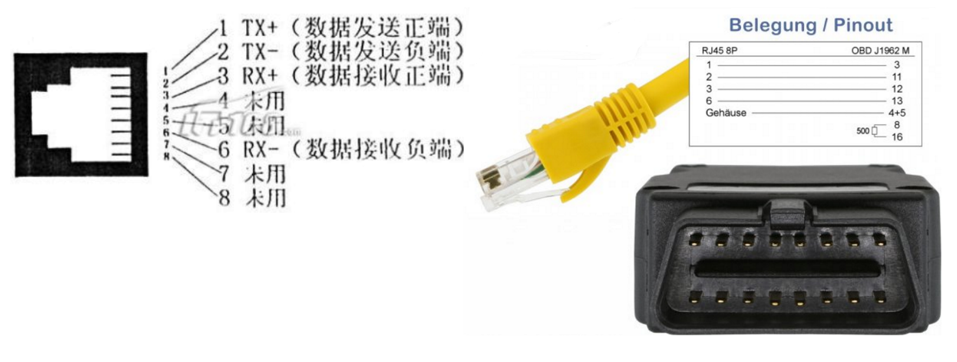
\includegraphics[scale=0.6]{pic/Quicker_20211111_101031.png}
    \caption{obd-RJ45 pin脚定义}
    \label{fig:Quicker_20211111_101031}
\end{figure}

\begin{figure}[ht]
    \centering
    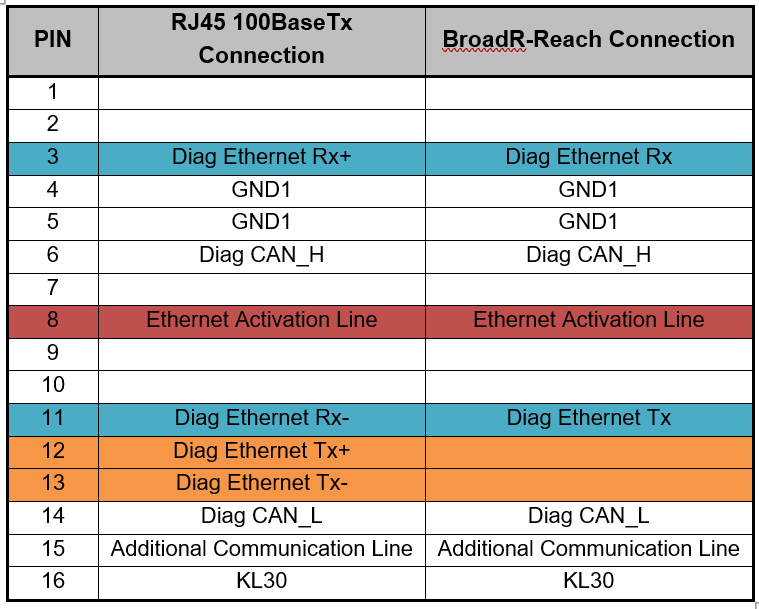
\includegraphics[scale=0.6]{pic/obd_pin.png}
    \caption{obd pin脚定义}
    \label{fig:obd_pin}
\end{figure}

\begin{figure}[ht]
    \centering
    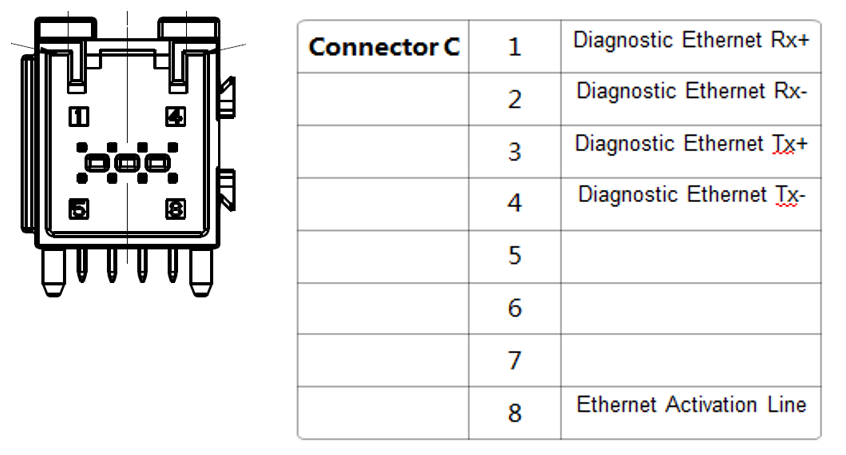
\includegraphics[scale=0.6]{pic/connect_c_pin.png}
    \caption{Connect C pin脚定义}
    \label{fig:connect_c_pin}
\end{figure}

通过如上接线,可实现pc网卡和GW诊断接口的以太网连接,由于RJ45-OBD16的以太网激活线(pin8)和kl30(pin16)经电阻直连,所以实车插入obd后,即可激活DoIP。台架上则需注意供电或直接拉高以太网激活线。

\subsection{Switch端口镜像配置方法}

Switch的端口镜像功能实现将某一指定Port的入口流量(ingress)和出口流量(egress)镜像至另一指定Port,便于switch流量的实时监控。以太网硬件诊断需求中使用DID CE06配置使能switch A各端口的镜像功能,输出镜像流量的Port为Switch A的port6,即本地诊断口。

\begin{figure}[ht]
    \centering
    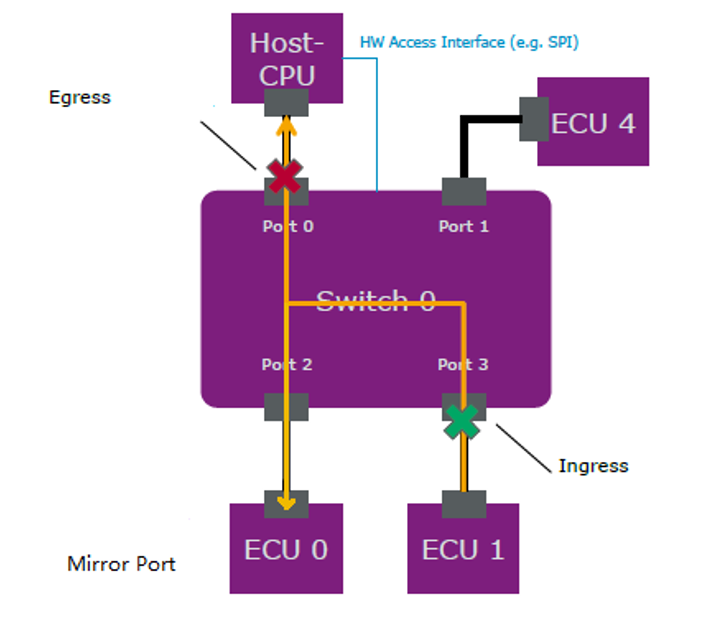
\includegraphics[scale=0.6]{pic/switch_mirror.png}
    \caption{switch端口镜像功能}
    \label{fig:switch_mirror}
\end{figure}

DID CE06共两字节,各bit控制信息如下表所示:

% Table generated by Excel2LaTeX from sheet 'Sheet1'
\begin{table}[htbp]
    \centering
    \caption{Add caption}
      \begin{tabular}{ccp{7.165em}p{7.165em}p{8.125em}}
      \toprule
      \rowcolor[rgb]{ .651,  .651,  .651} \multicolumn{1}{p{2.585em}}{\textbf{Byte}} & \multicolumn{1}{p{3.71em}}{\textbf{Bite}} & \textbf{Switch port} & \textbf{对应控制器\newline{}(硬件0.66)} & \textbf{对应控制器\newline{}(硬件0.66之前版本)} \\
      \midrule
      1     & 7     & \multicolumn{1}{c}{1} & Rev   & Tbox    0x8000 \\
      1     & 6     & \multicolumn{1}{c}{2} & Tbox    0x4000 & Lads    0x0400 \\
      1     & 5     & \multicolumn{1}{c}{3} & Icm     0x2000 & Rev \\
      1     & 4     & \multicolumn{1}{c}{4} & Fvcm    0x1000 & Icm     0x1000 \\
      1     & 3     & \multicolumn{1}{c}{5} & Lads    0x0800 & Fvcm    0x0800 \\
      1     & 2     & Rev   & Rev   & Rev \\
      1     & 1     & Rev   & Rev   & Rev \\
      1     & 0     & Rev   & Rev   & Rev \\
      2     & 7     & Rev   & Rev   & Rev \\
      \bottomrule
      \end{tabular}%
    \label{tab:addlabel}%
\end{table}%

通过2E服务写入CE06指定配置并复位后,即可开启指定端口的镜像功能。不同硬件Switch各端口的对应关系如下图所示:

\begin{figure}[ht]
    \centering
    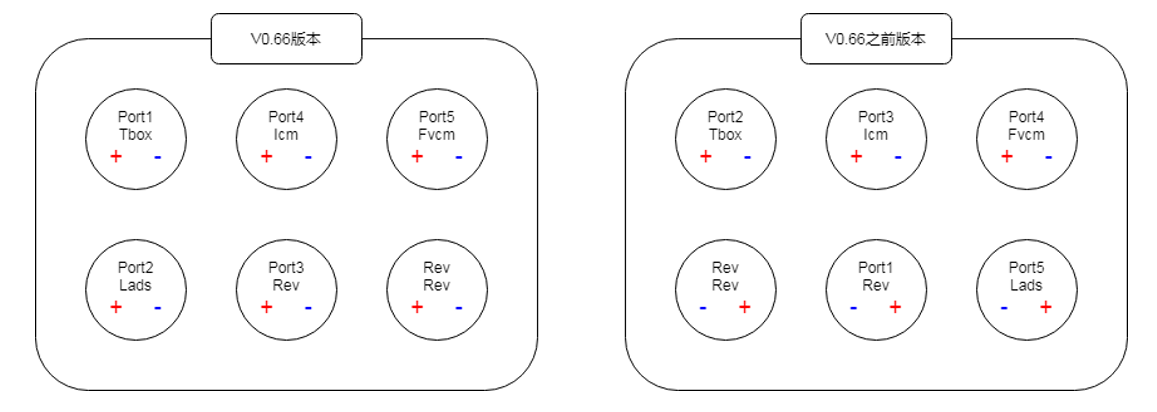
\includegraphics[scale=0.6]{pic/two_version_hardware_mapping.png}
    \caption{}
    \label{fig:two_version_hardware_mapping}
\end{figure}

通过31服务执行RID FE10,即可通过GW ping其他节点,以检测以太网链路是否正常。
如ping Tbox(172.31.7.21)命令如下:

\begin{lstlisting}
    >  Tx: 31 01 FE 10 01 AC 1F 07 15
\end{lstlisting}

